\documentclass[12pt]{article}
\usepackage{graphicx}
\usepackage[section]{placeins}
\usepackage{amsmath}
\usepackage{listings}
\usepackage{xcolor}

\usepackage[top=1.0in, bottom=1.0in, left=0.5in, right=0.5in]{geometry}
\renewcommand{\thesection}{}
\renewcommand{\thesubsection}{\arabic{subsection}}
\lstdefinelanguage{VHDL}{
  morekeywords={
    library,use,all,entity,is,port,in,out,end,architecture,of,
    begin,and,case,when,process,ALL,downto,Port,null,others
  },
  morekeywords=[2]{
    STD_LOGIC_VECTOR,STD_LOGIC,IEEE,STD_LOGIC_1164,
    NUMERIC_STD,STD_LOGIC_ARITH,STD_LOGIC_UNSIGNED,std_logic_vector,
    std_logic
  },
  morecomment=[l]--
}
\colorlet{keyword}{blue!100!black!80}
\colorlet{comment}{green!90!black!100}
\colorlet{STD}{red!100!white!80}
\colorlet{background}{white!100!black!100}
\lstdefinestyle{vhdl}{
  language     = VHDL,
  basicstyle   = \ttfamily,
  keywordstyle = [1]\color{keyword}\bfseries,
  keywordstyle = [2]\color{STD}\bfseries,
  commentstyle = \color{comment},
}
\lstset{
	frame = single,
	backgroundcolor = \color{background},
	numbers = left,
	captionpos = b,
	stringstyle = \ttfamily\color{red!50!brown}
}

\begin{document}
\title{\vspace{15ex}\Huge{CS 288:\\ BCD to 7 Segment Decoder \\ \& \\ Pseudo Random Number Generator}\vspace{15ex}}


\author{
  Dheerendra Singh Rathor\\120050033\\
  \texttt{dheeru.rathor14@gmail.com}\\[1 cm]
}

\date{\today}
\maketitle
\newpage

\section{Aim:}
Using Xilinix ISE Tools to simulate BCD to 7 Segment decoder and Pseudo Random Number Generator using behavioral model.

\section{Procedure:}
The procedure for 7 Segment decoder and Pseudo Random Number Generator is given in the following subsections respectively
\subsection{BCD to 7 Segment Decoder}
For making BCD to 7 Segment Decoder, I used to logic vectors viz. bcd and ouput respectively 3 downto 0 and 6 downto 0. 
\begin{figure}[!ht]
\centering
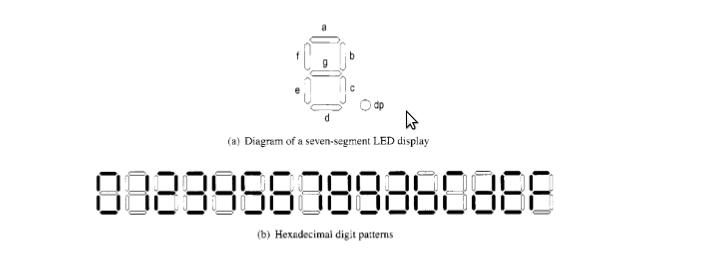
\includegraphics[scale=0.5]{pic}
\end{figure}
Logic vector output is taken as "gfedcba". \\
Values to each case is given using the truth table given below.
\begin{center}
\begin{tabular}{| l | l | l | l |}
\hline
S. No. & output value & bcd & output vector \\ \hline
1. & 0 & 0000 & 0111111 \\ \hline
2. & 1 & 0001 & 0000110 \\ \hline
3. & 2 & 0010 & 1011011 \\ \hline
4. & 3 & 0011 & 1001111 \\ \hline
5. & 4 & 0100 & 1100110 \\ \hline
6. & 5 & 0101 & 1101101 \\ \hline
7. & 6 & 0110 & 1111101 \\ \hline
8. & 7 & 0111 & 0000111 \\ \hline
9. & 8 & 1000 & 1111111 \\ \hline
10. & 9 & 1001 & 1101111 \\ \hline
11. & a & 1010 & 1011111 \\ \hline
12. & b & 1011 & 1111100 \\ \hline
13. & c & 1100 & 0111001 \\ \hline
14. & d & 1101 & 1011110 \\ \hline
15. & e & 1110 & 1111001 \\ \hline
16. & f & 1111 & 1110001 \\ \hline
\end{tabular}
\end{center}
This code is written in sequential behaviour using case when statements. 
Timing diagrams and code are included in coming sections.
\subsection {Pseudo Random Number Generator}
Pseudo Random Number Generator is written using 1 generator variable named "gen". 1 output vector named output which is the random number vector. and two incode variable are used as output\_temp and temp.\\
if gen is 1 then output will be a random value. 
\\
This code is written in sequential behaviour using case - when statement. Timing diagram and code are included in coming 
sections. 
\section{Timing Diagrams}
\begin{figure}[!ht]
\centering
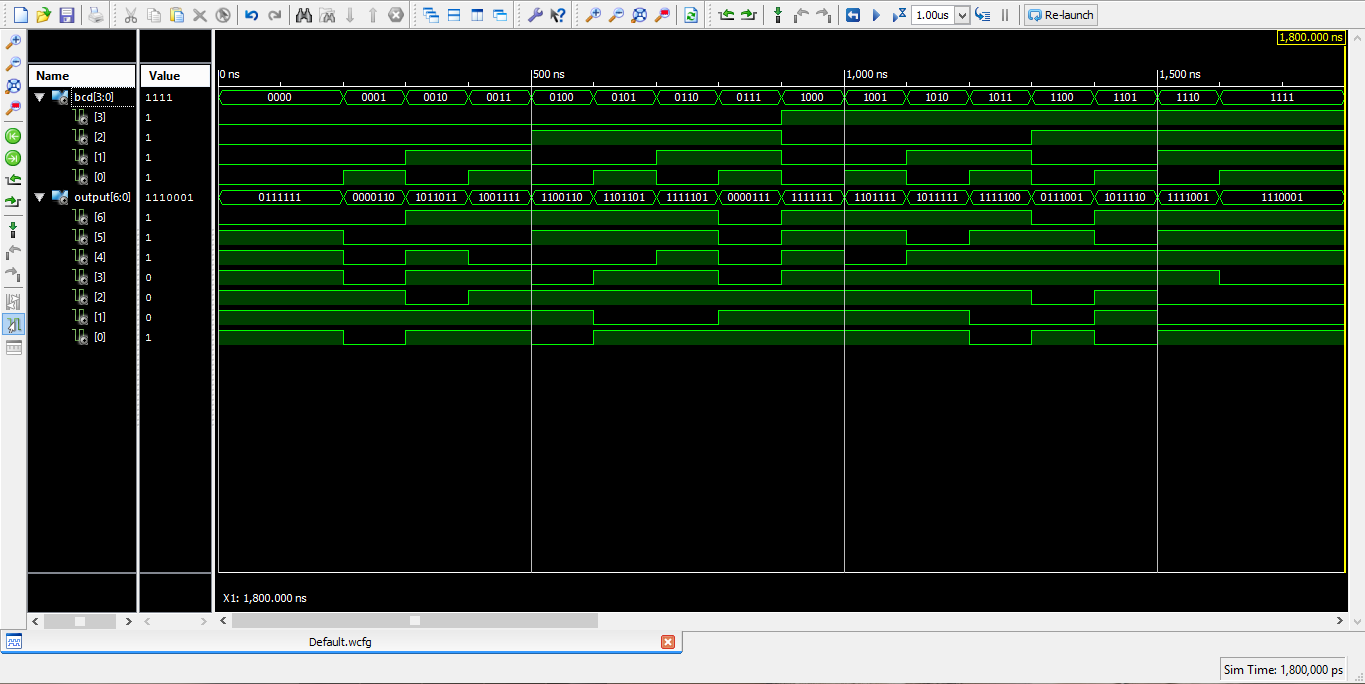
\includegraphics[scale=0.5]{bcd-segment}
\caption{Timing Diagram for 7 segment decoder from 0ns to 1800 ns}
\label{fig1}
\end{figure}
\newpage
\begin{figure}[!ht]
\centering
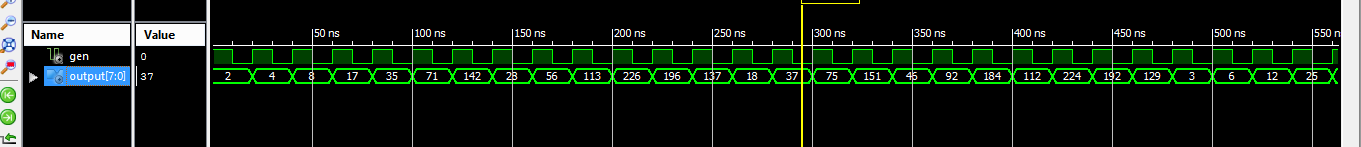
\includegraphics[scale=0.5]{Capture}
\end{figure}
\begin{figure}[!ht]
\centering
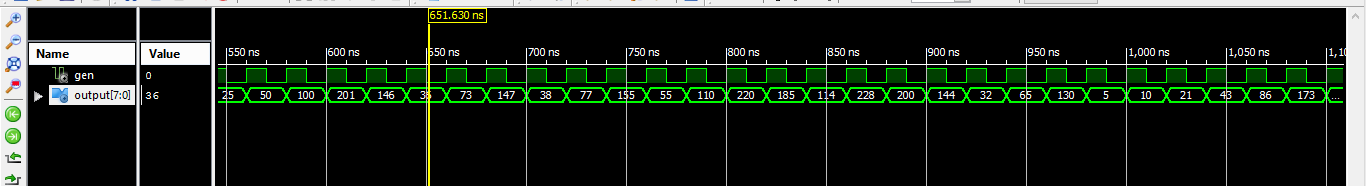
\includegraphics[scale=0.5]{Capture1}
\end{figure}
\begin{figure}[!ht]
\centering
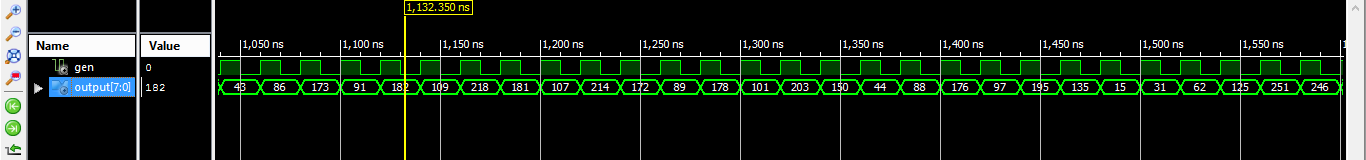
\includegraphics[scale=0.5]{Capture2}
\end{figure}
\begin{figure}[!ht]
\centering
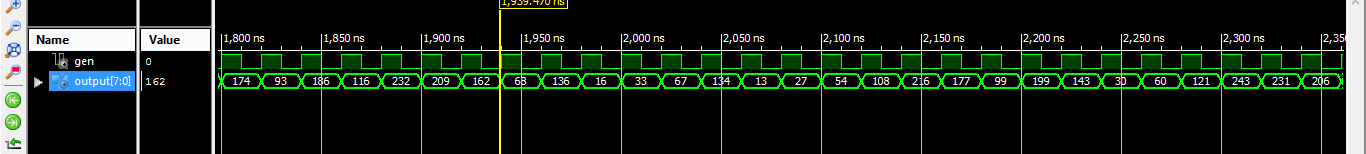
\includegraphics[scale=0.5]{Capture3}
\end{figure}
\begin{figure}[!ht]
\centering
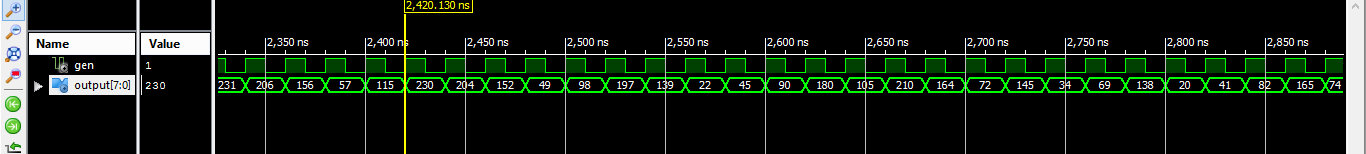
\includegraphics[scale=0.5]{Capture4}
\end{figure}
\begin{figure}[!ht]
\centering
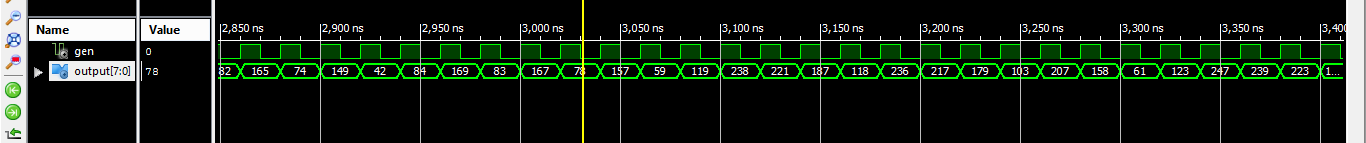
\includegraphics[scale=0.5]{Capture5}
\end{figure}
\begin{figure}[!ht]
\centering
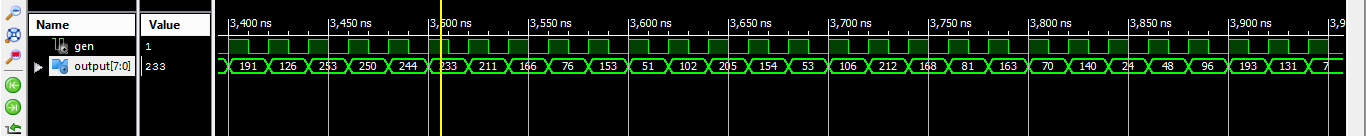
\includegraphics[scale=0.5]{Capture6}
\end{figure}
\begin{figure}[!ht]
\centering
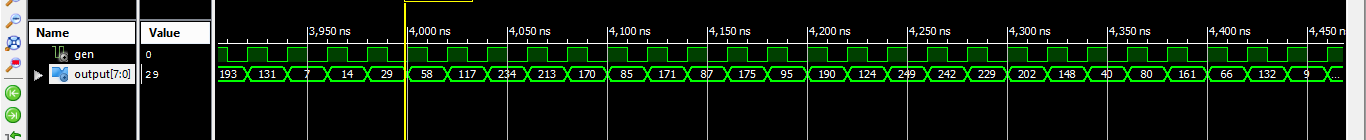
\includegraphics[scale=0.5]{Capture7}
\end{figure}
\begin{figure}[!ht]
\centering
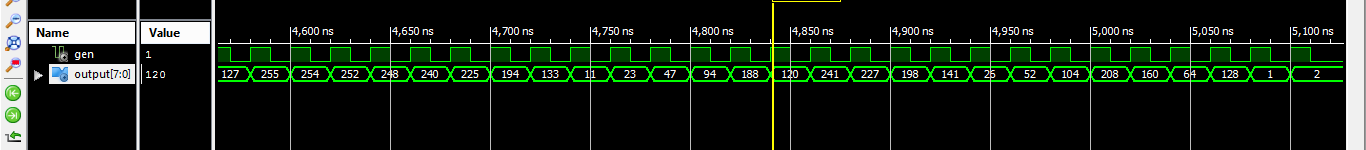
\includegraphics[scale=0.5]{Capture8}
\caption{Timing Diagrams for pseudo random number generator}
\label{fig2}
\end{figure}
\newpage
\section{Codes}
Here I have include working code for both BCD to 7 segment Decoder and Pseudo Random Number Generator
\subsection{code for BCD to 7 segment Decoder}
\begin{lstlisting}[style=vhdl]
----------------------------------------------------------------------------------
-- Company: 
-- Engineer: 
-- 
-- Create Date:    14:23:10 02/25/2014 
-- Design Name: 
-- Module Name:    bcd_7_segment - Behavioral 
-- Project Name: 
-- Target Devices: 
-- Tool versions: 
-- Description: 
--
-- Dependencies: 
--
-- Revision: 
-- Revision 0.01 - File Created
-- Additional Comments: 
--
----------------------------------------------------------------------------------
library IEEE;
use IEEE.STD_LOGIC_1164.ALL;

-- Uncomment the following library declaration if using
-- arithmetic functions with Signed or Unsigned values
--use IEEE.NUMERIC_STD.ALL;

-- Uncomment the following library declaration if instantiating
-- any Xilinx primitives in this code.
--library UNISIM;
--use UNISIM.VComponents.all;

entity bcd_7_segment is
    Port ( bcd : in  STD_LOGIC_VECTOR (3 downto 0);
           output : out  STD_LOGIC_VECTOR (6 downto 0));
end bcd_7_segment;

architecture Behavioral of bcd_7_segment is
begin process (bcd)
begin
output <= "0000000";
case bcd is
	when "0000" =>
		output <= "0111111";
	when "0001" =>
		output <= "0000110";
	when "0010" =>
		output <= "1011011";
	when "0011" =>
		output <= "1001111";
	when "0100" =>
		output <= "1100110";
	when "0101" =>
		output <= "1101101";
	when "0110" =>
		output <= "1111101";
	when "0111" =>
		output <= "0000111";
	when "1000" =>
		output <= "1111111";
	when "1001" =>
		output <= "1101111";
	when "1010" =>
		output <= "1011111";
	when "1011" =>
		output <= "1111100";
	when "1100" =>
		output <= "0111001";
	when "1101" =>
		output <= "1011110";
	when "1110" =>
		output <= "1111001";
	when "1111" =>
		output <= "1110001";
	when others =>
		null;

end case;
end process;

end Behavioral;

\end{lstlisting}

\subsection{Code for Pseudo Random Number Generator}
\begin{lstlisting}[style=vhdl]
----------------------------------------------------------------------------------
-- Company: 
-- Engineer: 
-- 
-- Create Date:    15:15:18 02/25/2014 
-- Design Name: 
-- Module Name:    rand - Behavioral 
-- Project Name: 
-- Target Devices: 
-- Tool versions: 
-- Description: 
--
-- Dependencies: 
--
-- Revision: 
-- Revision 0.01 - File Created
-- Additional Comments: 
--
----------------------------------------------------------------------------------
library IEEE;
use IEEE.STD_LOGIC_1164.ALL;

-- Uncomment the following library declaration if using
-- arithmetic functions with Signed or Unsigned values
--use IEEE.NUMERIC_STD.ALL;

-- Uncomment the following library declaration if instantiating
-- any Xilinx primitives in this code.
--library UNISIM;
--use UNISIM.VComponents.all;

entity rand is
    Port ( gen : in  STD_LOGIC;
           output : out  STD_LOGIC_VECTOR (7 downto 0));
end rand;

architecture Behavioral of rand is
begin process(gen)
variable output_temp : std_logic_vector( 7 downto 0) := "00000001";
variable temp :std_logic := '0';
begin
case gen is
	when '1' =>
		temp := output_temp(7) xor output_temp(5) xor output_temp(4) xor output_temp(3);
		output_temp(7 downto 1) := output_temp(6 downto 0);
		output_temp(0) := temp;
		output <= output_temp;
	when others =>
		null;
end case;
end process;


end Behavioral;

\end{lstlisting}

\section{Inference}
In this assignment I infered the followings:\\
\verb|1.| Working of BCD to 7 segment decoder \\
\verb|2.| Truth table for bcd to 7 segment decoder \\
\verb|3.| Using for loop in VHDL \\
\verb|4.| Generating random numbers using hardware tools \\
\end{document}
